\subsection{Radiation and Relativistic Dynamics}

\subsubsection{Emission Rates by Lorentz Transformation}\label{Emission Rates by Lorentz Transformation}

In the (momentary) rest frame of the electron, the particle acceleration is given by $F' = m a^{\prime}=e E^{\prime} $ and Larmor's formula gives the exact rate at which the particle radiates energy:

\begin{equation}
	P^{\prime}=\frac{d U^{\prime}}{d t^{\prime}}=\frac{1}{4 \pi \epsilon_{0}} \frac{2 e^{2}}{3 c^{3}} \left(\frac{dp'}{dt'}\right)^{2}=\frac{1}{4 \pi \epsilon_{0}} \frac{2 e^{2}}{3 c^{3}} \frac{e^{2} E^{\prime 2}}{m^{2}}.
\end{equation}

\begin{figure}[h]
	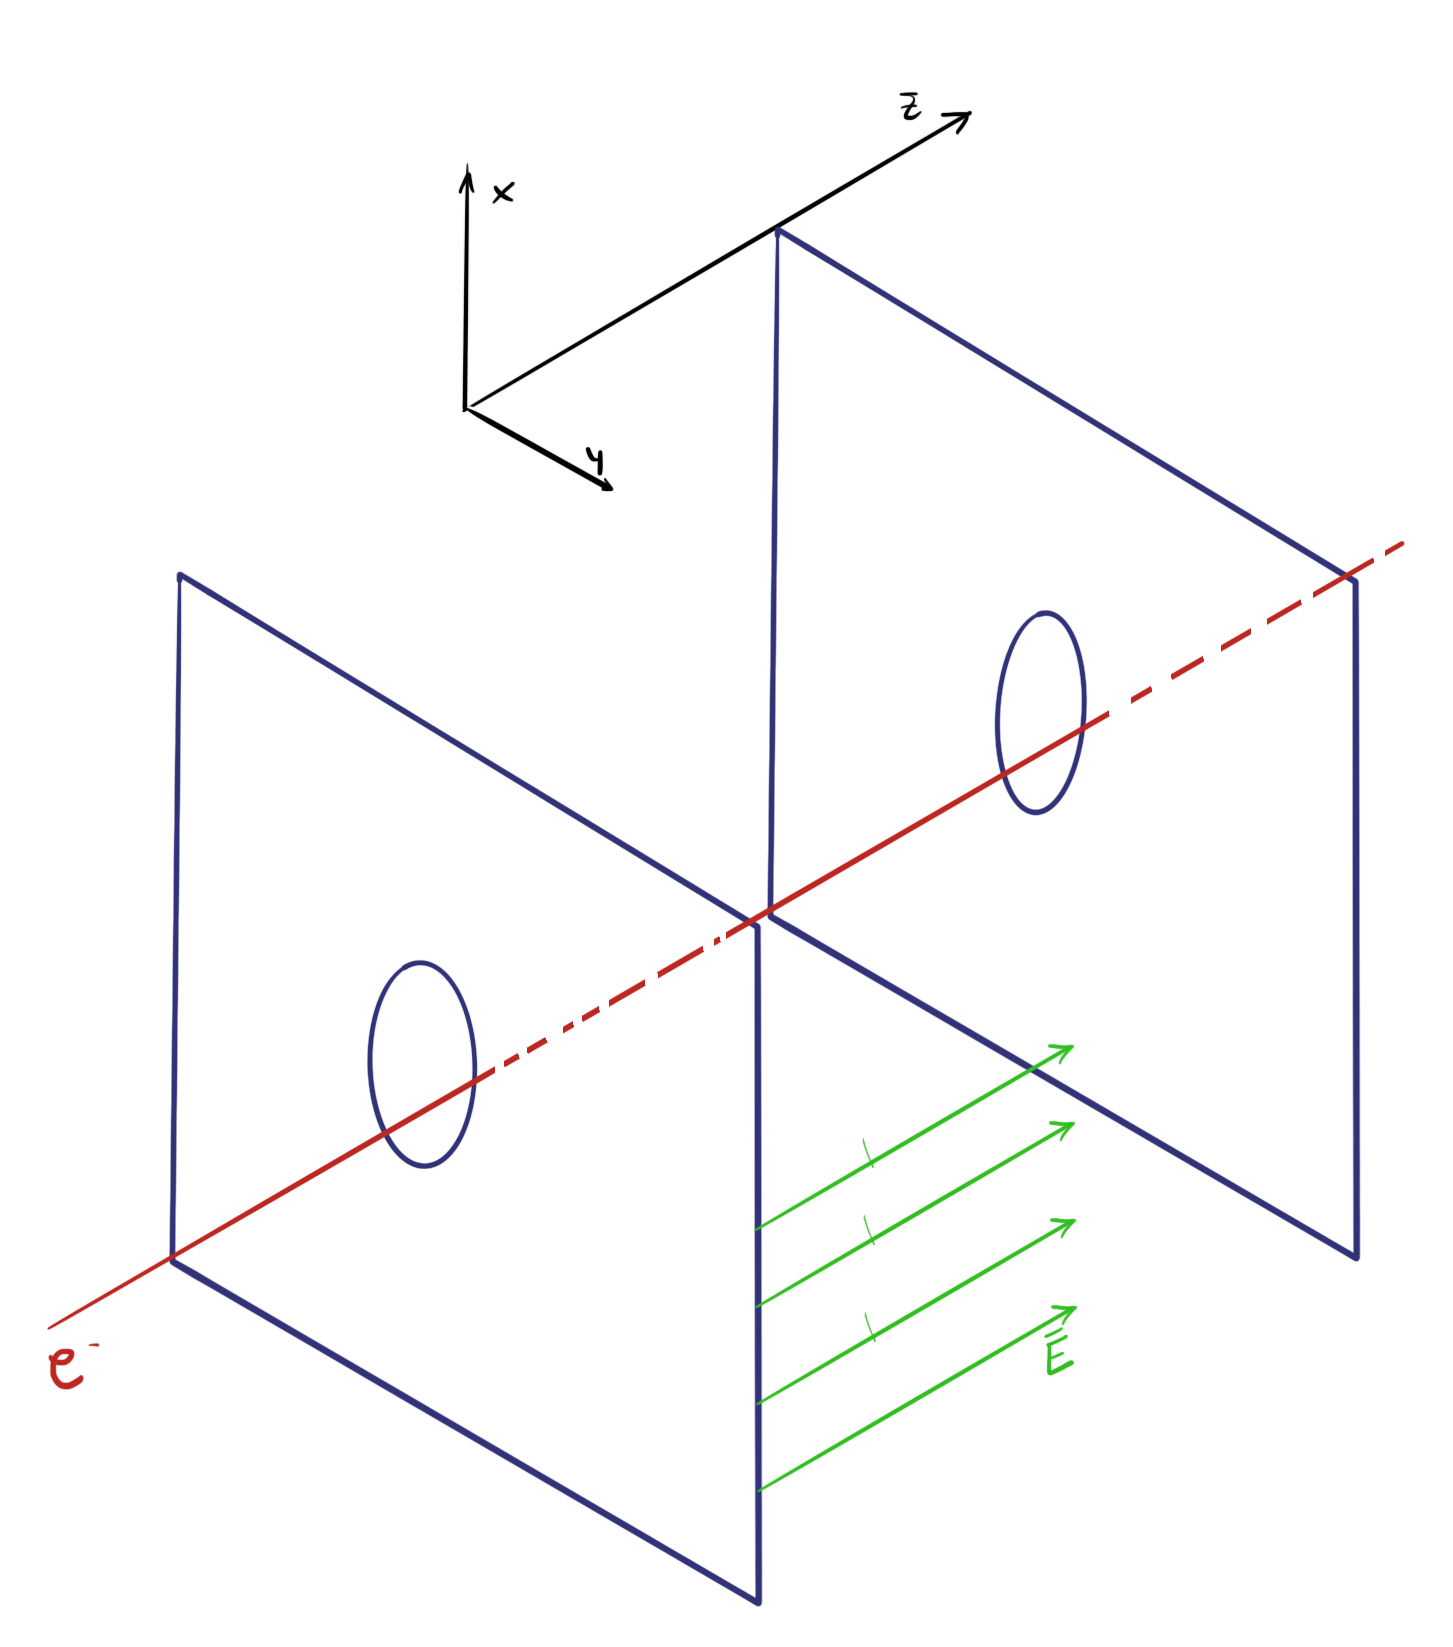
\includegraphics[width=6cm]{figures/EmissionRates.png}
	\centering
	\caption{The system we want to study.}
\end{figure}

Therefore, the total energy lost to radiation (recall that $P = \tfrac{E}{t}$ and there is no change in $\vec{v}$ of the $e^{-}$) is;

\begin{equation}
	\Delta U^{\prime}=P^{\prime} t^{\prime}=\frac{1}{4 \pi \epsilon_{0}} \frac{2 e^{4} E^{\prime 2} t^{\prime}}{3 m^{2} c^{3}}
\end{equation}

We have to realise that there is no preferred direction in the rest frame, so $\Delta P^{\prime}=0$. Transforming to the laboratory frame,

\begin{equation}
		\Delta U = \gamma \Delta U' = \gamma \sqrt{\Delta U'^{2} + \cancel{\Delta P^{2}}} = \gamma \frac{1}{4 \pi \epsilon_{0}} \frac{2 e^{4} E^{\prime 2} t^{\prime}}{3 m^{2} c^{3}}.
	\end{equation}

The electric field $\ve$ is parallel to the boost, so $E=E^{\prime}$. The electron transit time through the capacitor is $t=d / v$ and $t=\gamma t^{\prime}$ by time dilation. Therefore,

\begin{equation}
	\Delta U=\gamma \frac{1}{4 \pi \epsilon_{0}} \frac{2 e^{4} E^{\prime 2} t^{\prime}}{3 m^{2} c^{3}}=\frac{1}{4 \pi \epsilon_{0}} \frac{2 e^{4} E^{2} d}{3 m^{2} c^{3} v}.
\end{equation}

The associated total momentum radiated is

\begin{equation}
	\Delta P=\gamma\left(\cancel{\Delta P^{\prime}}+v \Delta U^{\prime} / c^{2}\right)=\frac{\gamma v \Delta U^{\prime}}{c^{2}}=\frac{v \Delta U}{c^{2}}=\frac{1}{4 \pi \epsilon_{0}} \frac{2 e^{4} E^{2} d}{3 m^{2} c^{5}}.
\end{equation}

\subsubsection{A Merry Go Round of Radiating Particles}\label{A Merry Go Round of Radiating Particles}

For a single charged particle, the Liénard-Wiechert electric field is:

\begin{equation}
	\mathbf{E}(\mathbf{r}, t)=\frac{q}{4 \pi \epsilon_{0}}\left[\underbrace{\frac{(\hat{\mathbf{n}}-\boldsymbol{\beta})}{\gamma^{2}(1-\hat{\mathbf{n}} \cdot \boldsymbol{\beta})^{3} R^{2}}}_{\text{Static fields $\propto \: 1/R^{2}$}}+\underbrace{\frac{\hat{\mathbf{n}} \times\{(\hat{\mathbf{n}}-\boldsymbol{\beta}) \times \dot{\boldsymbol{\beta}}\}}{c(1-\hat{\mathbf{n}} \cdot \boldsymbol{\beta})^{3} R}}_{\text{Radiative fields $\propto \: 1/R$}}\right]_{\mathrm{ret}}
\end{equation}

Basically we have to prove that our final result only contains the first term. In order to do so, the first question we have to answer for this problem is: How does the set up look like? Observe the following sketch.

\begin{figure}[h!]
	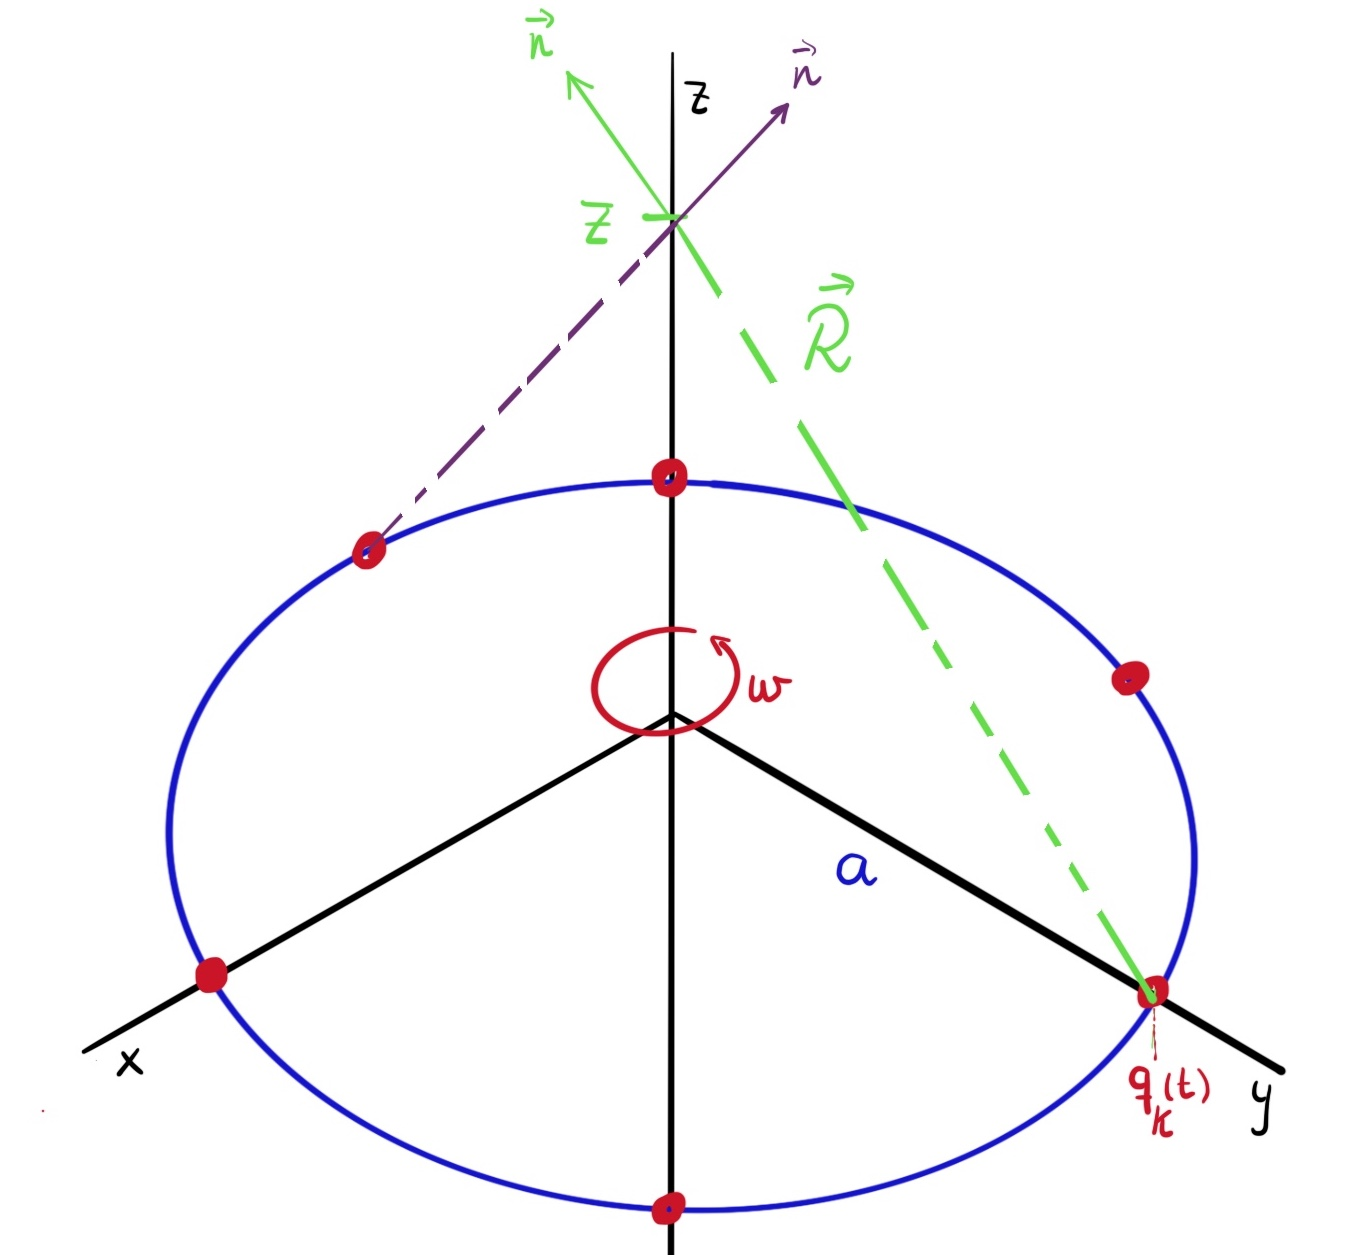
\includegraphics[width=8cm]{figures/AMerryGoRound.jpg}
	\centering
	\caption{A frame of the motion of N particles around an axis.}
\end{figure}

So we have to compute the position and velocity variables for a generic particle in this system. For simplicity, let us take the center of coordinates lying on the position $\vec{p}$ of the $z$ axis. So $\mathbf{R} (t)$ is given by:

\begin{equation}
	\mathbf{R}_{k}(t) = \vec{p} - \vec{q}_{k}(t) = -a \cos \left(\omega t+\phi_{k}\right) \hat{\mathbf{x}}-a \sin \left(\omega t+\phi_{k}\right) \hat{\mathbf{y}}+z \hat{\mathbf{z}},
\end{equation}

where $v=a \omega$ ($\omega$ is the angular velocity of these particles) and $\phi_{k}=2 \pi k / N$. From the sketch above, $R_{k}=\sqrt{a^{2}+z^{2}}=R$ is the same for all the particles and constant, so $\hat{n} = \mathbf{R}/ |\mathbf{R}|$. What is the velocity? And the acceleration?

\begin{equation}
	\begin{split}
			\boldsymbol{\beta}_{k}&= -\frac{\partial \mathbf{q}_{k}}{c \: \partial t}=\beta\left[-\sin \left(\omega t+\phi_{k}\right) \hat{\mathbf{x}}+\cos \left(\omega t+\phi_{k}\right) \hat{\mathbf{y}}\right], \\
			\dot{\boldsymbol{\beta}}_{k}&= -\frac{\partial \boldsymbol{\beta}_{k}}{ \: \partial t}= -\omega \beta\left[\cos \left(\omega t+\phi_{k}\right) \hat{\mathbf{x}}+\sin \left(\omega t+\phi_{k}\right) \hat{\mathbf{y}}\right].
	\end{split}
\end{equation}

Step by step, we get closer to the solution. Now, we have to compute the scalar and vector products as:

\begin{equation}
	\begin{split}
		&\hat{\mathbf{n}}_{k} \cdot \boldsymbol{\beta}_{k}= ( -\tfrac{a}{|\mathbf{R}|} \cos \left(\dots\right), -\tfrac{a}{|\mathbf{R}|} \sin \left(\dots\right) , z )\cdot (-\beta \sin \left(\dots\right), \beta \cos \left(\dots\right) ,0)  =0,\\
		&\hat{\mathbf{n}}_{k} \times\left(\left(\hat{\mathbf{n}}_{k}-\boldsymbol{\beta}\right) \times \dot{\boldsymbol{\beta}}\right)= \underbrace{\left(\hat{\mathbf{n}}_{k}-\boldsymbol{\beta}\right)\left(\hat{\mathbf{n}}_{k} \cdot \dot{\boldsymbol{\beta}}\right)-\dot{\boldsymbol{\beta}}}_{\vec{a}\times \vec{b}\times\vec{c} = b (\vec{a}\cdot \vec{c})- c (\vec{a}\cdot \vec{b})}.
	\end{split}
\end{equation}

Where:

\begin{equation}
	\left(\hat{\mathbf{n}}_{k} \cdot \dot{\boldsymbol{\beta}}\right) = \frac{c \boldsymbol{\beta}^{2}}{|\mathbf{R}|}.
\end{equation}

And $\left(\hat{\mathbf{n}}_{k}-\boldsymbol{\beta}\right)$ is left untouched for convenience. Then, after some computation we have all the necessary terms to compute the electric field, which is given by:

\begin{equation}\label{almost}
	\mathbf{E}(z, t)=\frac{q}{4 \pi \epsilon_{0}} \sum_{k=1}^{N}\left[\frac{\left(\hat{\mathbf{n}}_{k}-\boldsymbol{\beta}_{k}\right)}{R^{2}}\left(\underbrace{\frac{1}{\gamma^{2}}+\beta^{2}}_{\text{$=1$}}\right)-\frac{\dot{\boldsymbol{\beta}}_{k}}{c R}\right]_{\mathrm{ret}}=\frac{q}{4 \pi \epsilon_{0}} \sum_{k=1}^{N}\left[\frac{\left(\hat{\mathbf{n}}_{k}-\boldsymbol{\beta}_{k}\right)}{R^{2}}-\frac{\dot{\boldsymbol{\beta}}_{k}}{c R}\right]_{\mathrm{ret}}.
\end{equation}

At this point of the problem, we need to realise something. The $x$ - and $y$ -components of this electric field vanish because, when $N>1$,

\begin{equation}
	\sum_{k=1}^{N} \cos \left(\omega t+\phi_{k}\right)=\sum_{k=1}^{N} \sin \left(\omega t+\phi_{k}\right)=0.
\end{equation}

The proof that both sums vanish is something as:

\begin{equation}
	\sum_{k=1}^{N} e^{i\left(\omega t+\phi_{k}\right)}=e^{i(\omega t+2 \pi / N)} \sum_{k=1}^{N} e^{i(k-1) 2 \pi / N}=e^{i(\omega t+2 \pi / N)} \frac{1-e^{i 2 \pi}}{1-e^{i 2 \pi / N}}=0.
\end{equation}

One can also see this vanishing by considering an even\footnote{In the case of odd number, one can take 3 particles and check that the sum of 2 of the $i$-components correspond to the remaining one with oposite sign.} number of particles. In this case, by the radial symmetry in the system, each vector $\mathbf{R}_{k}$ will have a "counter" vector $\mathbf{R}_{-k}$, whose $\hat{x}$ and $\hat{y}$ components will have opposite sign of the $k$ vector ones. So the only term in (\ref{almost}) which survives is the $z$ -component of $\hat{\mathbf{n}}_{k} .$ Hence, the electric field on the symmetry axis is:

\begin{equation}
	\mathbf{E}(z, t)=\hat{z} \frac{q}{4 \pi \epsilon_{0}} \sum_{k=1}^{N}\left[\frac{z}{R^{3}}\right]_{\mathrm{ret}}=\frac{q N z}{4 \pi \epsilon_{0} R^{3}} \hat{\mathrm{z}} \quad(N>1).
\end{equation}

Which has not time component involved, neither explicit nor implicit. This indicates a static configuration of the electric field.

\subsubsection{The Direction of the Velocity Field}\label{The Direction of the Velocity Field}

The velocity field is given by:

\begin{equation}
	\mathrm{E}=\frac{q}{4 \pi \epsilon_{0}}\left[\frac{\hat{\mathbf{n}}-\boldsymbol{\beta}}{\gamma^{2} g^{3} R^{2}}\right]_{\mathrm{ret}}
\end{equation}

And the direction of this field is the same as the direction of the vector,

\begin{equation}
	[\mathbf{R}-\boldsymbol{\beta}R]_{\mathrm{ret}}=\mathrm{r}-\mathrm{r}_{0}\left(t_{\mathrm{ret}}\right)-\boldsymbol{\beta}\left|\mathrm{r}-\mathrm{r}_{0}\left(t_{\mathrm{ret}}\right)\right|.
\end{equation}

For our convenience, let the observer sit at the origin $(\mathrm{r}=0)$. Then, because the retarded time is defined as:

\begin{equation}
	t_{\mathrm{ret}}+r_{0}\left(t_{\mathrm{ret}}\right) / c-t=0,
\end{equation}

the velocity electric field can be expressed as:

\begin{equation}
	\begin{split}
			\mathbf{E} \propto-\mathrm{r}_{0}\left(t_{\text {ret }}\right)-\frac{\mathbf{v}\left(t_{\text {ret }}\right)}{c} r_{0}\left(t_{\text {ret }}\right) &=-\mathbf{r}_{0}\left(t_{\text {ret }}\right)-\mathbf{v}\left(t_{\text {ret }}\right)\left(t-t_{\text {ret }}\right)= \\
		&=-\left[\mathbf{r}_{0}\left(t_{\text {ret }}\right)+\mathbf{v}\left(t_{\text {ret }}\right)\left(t-t_{\text {ret }}\right)\right]=-\mathbf{r}_{A} .
	\end{split}
\end{equation}

The diagram below shows that this proves the assertion.
\begin{figure}[h!]
	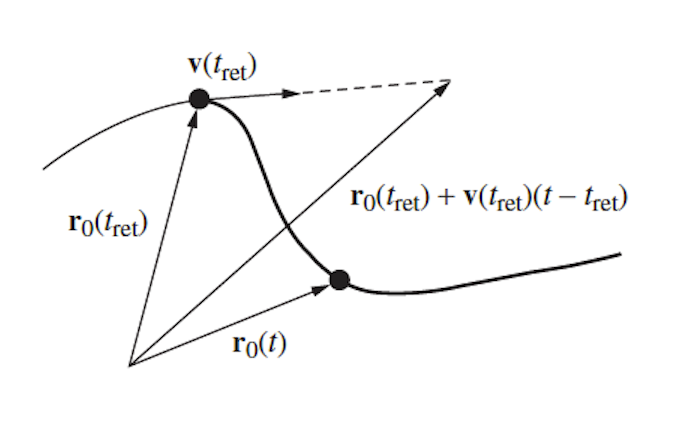
\includegraphics[width=8cm]{figures/DirectionVelocityField.png}
	\centering
\end{figure}

\subsubsection{Radiating 14.4 Jackson Problem}\label{Radiating 14.4 Jackson Problem}

\textbf{a):}

In the non-relativistic limit, the radiated power is given by

\begin{equation}\label{radiatedpower}
	\frac{d P(t)}{d \Omega}=\frac{e^{2}}{4 \pi c}|\hat{n} \times \dot{\vec{\beta}}|^{2}.
\end{equation}

For this part of the problem, we just have to make the observation that the particle has an harmonic motion along the $z$ axis, so we take:

\begin{equation}
	\vec{r}=\hat{z} a \cos \omega_{0} t, \quad \vec{\beta}= \frac{\partial \vec{r}}{c\: \partial t} = -\hat{z} \frac{a \omega_{0}}{c} \sin \omega_{0} t, \quad \dot{\vec{\beta}}=-\hat{z} \frac{a \omega_{0}^{2}}{c} \cos \omega_{0} t.
\end{equation}

	
By symmetry, we can assume the observer is in the $x-z$ plane tilted with angle $\theta$ from the vertical. This means that we take the normal $\hat{n}$ to be:

\begin{equation}
	\hat{n}=\hat{x} \sin \theta+\hat{z} \cos \theta.
\end{equation}

Now we have all the ingredients to cook up the formula (\ref{radiatedpower}), so:

\begin{equation}
	\hat{n} \times \dot{\vec{\beta}}= \frac{a \omega_{0}^{2}}{c} \sin \theta \cos \omega_{0} t \: \hat{y}, \quad \Rightarrow \quad \frac{d P(t)}{d \Omega}=\frac{e^{2} a^{2} \omega_{0}^{4}}{4 \pi c^{3}} \sin ^{2} \theta \cos ^{2} \omega_{0} t.
\end{equation}

And then, taking a time average $\left(\cos ^{2} \omega_{0} t \rightarrow 1 / 2\right)$ this gives:

\begin{equation}
	\frac{d P}{d \Omega}=\frac{e^{2} a^{2} \omega_{0}^{4}}{8 \pi c^{3}} \sin ^{2} \theta.
\end{equation}

To get the total power radiated, we just have to integrate over the solid angle $\Omega$, resulting:

\begin{equation}
	P=\frac{e^{2} a^{2} \omega_{0}^{4}}{3 c^{3}}.
\end{equation}

We can now plot how the radiated energy per solid angle looks like,

\begin{figure}[h]
	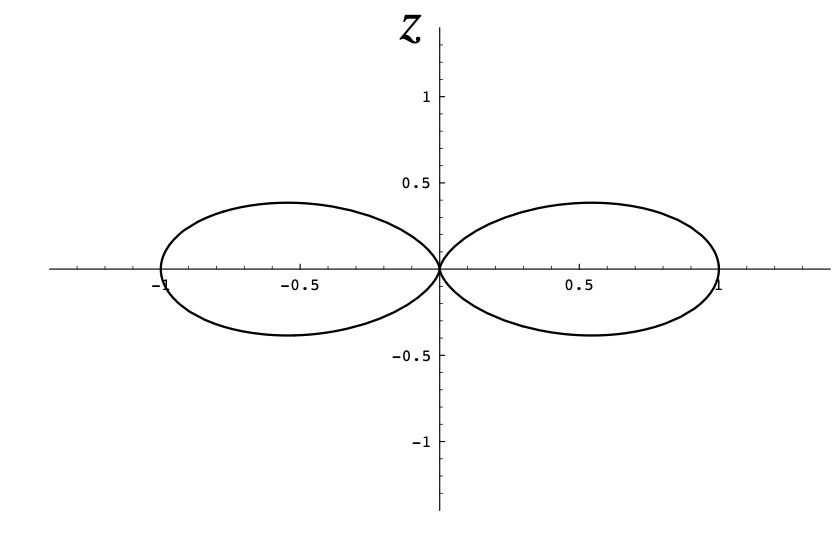
\includegraphics[width=8cm]{figures/RadiatingJackson1.png}
	\centering
	\caption{Distribution of the radiation for a bouncing particle.}
\end{figure}

\textbf{b):}

Now the particle decides to move along a circle of radius $R$ with constant angular frecuency $\omega_{0}$. This means that its position vector $\vec{r}$ is given by:

\begin{equation}
	\vec{r}=R\left(\hat{x} \cos \omega_{0} t+\hat{y} \sin \omega_{0} t\right).
\end{equation}

Therefore, the velocity and the acceleration derived from this previous expression are:

\begin{equation}
	\vec{\beta}=\frac{R \omega_{0}}{c}\left(-\hat{x} \sin \omega_{0} t+\hat{y} \cos \omega_{0} t\right) \quad \rightarrow \quad
	\dot{\vec{\beta}}=-\frac{R \omega_{0}^{2}}{c}\left(\hat{x} \cos \omega_{0} t+\hat{y} \sin \omega_{0} t\right).
	\end{equation}

Then, sitting at the same position as in the previous part of this exercise (a.k.a. same $\hat{n}$), one can find:

\begin{equation}
	\hat{n} \times \dot{\vec{\beta}}=-\frac{R \omega_{0}^{2}}{c}\left[ \cos \theta \cos \omega_{0} t \: \hat{y}+( \sin \theta \: \hat{z} - \cos \theta \: \hat{x}) \sin \omega_{0} t\right].
\end{equation}

And again, the distribution of radiation is:

\begin{equation}
	\frac{d P(t)}{d \Omega}=\frac{e^{2} R^{2} \omega_{0}^{4}}{4 \pi c^{3}}\left(\cos ^{2} \theta \cos ^{2} \omega_{0} t+\sin ^{2} \omega_{0} t\right).
\end{equation}

Taking time average gives:

\begin{equation}
	\frac{d P}{d \Omega}=\frac{e^{2} R^{2} \omega_{0}^{4}}{8 \pi c^{3}}\left(1+\cos ^{2} \theta\right).
\end{equation}

And the total radiation, after integrating is:

\begin{equation}
	P=\frac{2 e^{2} R^{2} \omega_{0}^{4}}{3 c^{3}}.
\end{equation}

In this case, the distribution of radiation across the solid angle is a little bit more involved, but easy to obtain using Mathematica or something similar.

\begin{figure}[h!]
	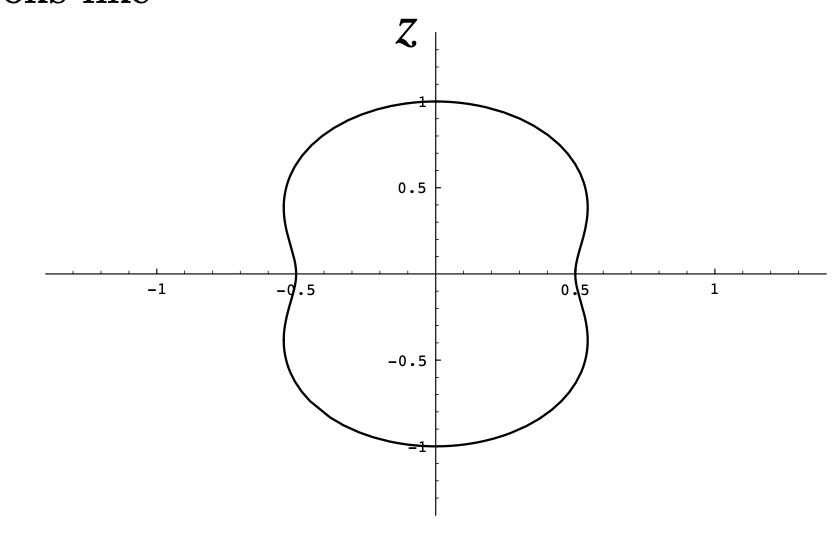
\includegraphics[width=8cm]{figures/RadiatingJackson2.png}
	\centering
	\caption{Distribution of the radiation for a particle in a circular motion.}
\end{figure}

\subsubsection{A Fast Particle in a Constant Electric Field}\label{A Fast Particle in a Constant Electric Field}

The equation of motion is the basic one for a charged particle moving in a constant field $\mathbf{E}$, as

\begin{equation}
	\frac{d \mathbf{p}}{d t}=q \mathbf{E} .
\end{equation}

\begin{figure}[h]
	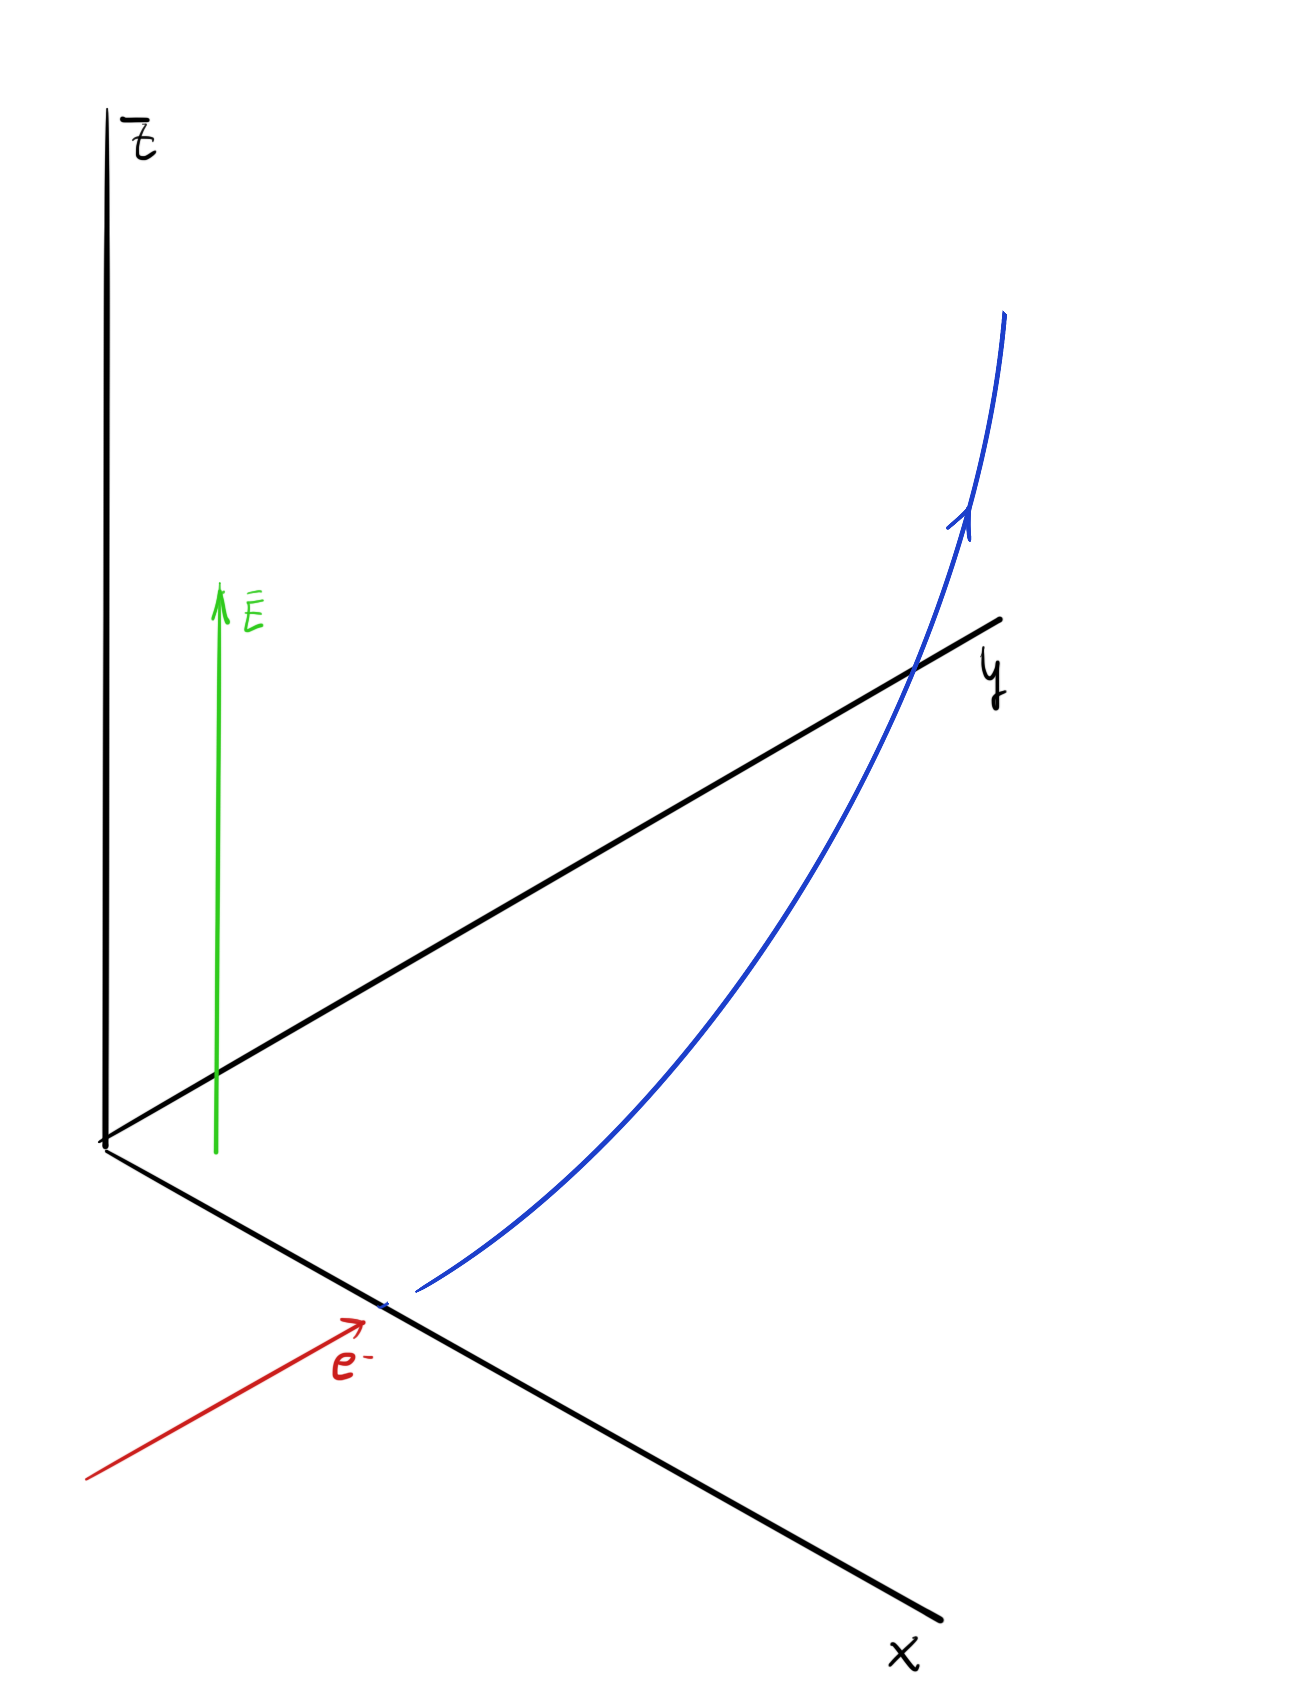
\includegraphics[width=5cm]{figures/FastParticle.png}
	\centering
	\caption{The motion of the particle within the field $\mathbf{E}$.}
\end{figure}\

With this, we can obtain the momentum of the particle depending on $t$. We just have to solve the differential equation imposing the initial condition $\mathbf{p}(0) = \gamma m u_{0} \hat{y}$. Then we have:

\begin{equation}
	\mathbf{p}(t)=p_{0} \hat{\mathbf{y}}+q E t \hat{\mathbf{z}}.
\end{equation}

The initial (total) energy of the particle is $\mathcal{E}_{0}=\sqrt{c^{2} p_{0}^{2}+m^{2} c^{4}}$. Therefore, the instantaneous velocity of the particle is:

\begin{equation}
	\mathbf{u}(t)=\frac{c^{2} \mathbf{p}}{\mathcal{E}}=\frac{c^{2} \mathbf{p}}{\sqrt{c^{2} p^{2}+m^{2} c^{4}}}=\frac{p_{0} \hat{\mathbf{y}}+q E t \hat{\mathbf{z}}}{\sqrt{\mathcal{E}_{0}^{2}+c^{2} q^{2} E^{2} t^{2}}} c^{2}.
\end{equation}

The particle speed goes $u \rightarrow c$ as $t \rightarrow \infty$. One can integrate the previous expression once respect to time to get $\mathbf{r}(t)$ as:

\begin{equation}
	\mathbf{r}(t)=\hat{\mathbf{y}} \frac{c p_{0}}{q E} \sinh ^{-1}\left(\frac{c q E t}{\mathcal{E}_{0}}\right)+\hat{\mathbf{z}} \frac{1}{q E} \sqrt{\mathcal{E}_{0}^{2}+c^{2} q^{2} E^{2} t^{2}} .
\end{equation}

The origin of coordinates so the integration constants are zero. Eliminating $t$ and using the properties of $\sinh x$ and $\cosh y$ we can arrive to the expected expression if:

\begin{equation}
	\begin{split}
		(x,y,z) &= \left(0, \frac{c p_{0}}{q E} \sinh ^{-1}\left(\frac{c q E t}{\mathcal{E}_{0}}\right),  \frac{1}{q E} \sqrt{\mathcal{E}_{0}^{2}+c^{2} q^{2} E^{2} t^{2}}\right) \rightarrow \\
		 &\\
		 \left(\frac{q E y}{c p_{0}}\right) &= \sinh ^{-1}\left(\frac{c q E t}{\mathcal{E}_{0}}\right), \quad \quad z =\frac{1}{q E} \sqrt{\mathcal{E}_{0}^{2}+c^{2} q^{2} E^{2} t^{2}}, \\
		 &\\
		 \cosh \left(\frac{q E y}{c p_{0}}\right) &= \cosh \left(\sinh ^{-1}\left(\frac{c q E t}{\mathcal{E}_{0}}\right)\right) = \sqrt{1 + \left(\frac{c q E t}{\mathcal{E}_{0}}\right)^{2}},\\
		 &\\
		\rightarrow z&=\frac{\mathcal{E}_{0}}{q E} \cosh \left(\frac{q E y}{c p_{0}}\right) .
	\end{split}
\end{equation}

The non-relativistic limit is $u \ll c$ or $c q E t \ll \mathcal{E}_{0}$. We recover the expected parabolic trajectory in this limit because $\cosh x \approx 1+\frac{1}{2} x^{2}$ when $x \ll 1$.

\subsubsection{A Ringy Radiating Problem}\label{A Ringy Radiating Problem}

\textbf{1):}

In the rest frame, $\varphi^{\prime}=0$ and

\begin{equation}
	\mathbf{A}^{\prime}\left(\mathbf{r}^{\prime}\right)=\frac{\mu_{0}}{4 \pi} \frac{\mathbf{m}^{\prime} \times \mathbf{r}^{\prime}}{r^{\prime 3}}.
\end{equation}

Therefore,

\begin{equation}
	\mathbf{A}_{\perp}^{\prime}=\frac{\mu_{0}}{4 \pi} \frac{\mathbf{m}_{\perp}^{\prime} \times \mathbf{r}_{\|}^{\prime}+\mathbf{m}_{\|}^{\prime} \times \mathbf{r}_{\perp}^{\prime}}{r^{\prime 3}}, \quad \quad \mathbf{A}_{\|}^{\prime}=\frac{\mu_{0}}{4 \pi} \frac{\mathbf{m}_{\perp}^{\prime} \times \mathbf{r}_{\perp}^{\prime}}{r^{\prime 3}} .
\end{equation}

On the other hand,

\begin{equation}
	\begin{split}
		\mathbf{A}_{\perp}&=\mathbf{A}_{\perp}^{\prime}, \\
		\mathbf{A}_{\|}&=\gamma\left(\mathbf{A}_{\|}^{\prime}+\mathbf{v}_{0} \varphi^{\prime} / c^{2}\right)=\gamma \mathbf{A}_{\|}^{\prime}, \\
		\varphi&=\gamma\left(\varphi^{\prime}+\mathbf{v}_{0} \cdot \mathbf{A}^{\prime}\right)=\gamma \mathbf{v}_{0} \cdot \mathbf{A}^{\prime} .
	\end{split}
\end{equation}

All together becomes,

\begin{equation}
	\begin{split}
		\mathbf{A}_{\perp}&=\frac{\mu_{0}}{4 \pi} \frac{\mathbf{m}_{\perp} \times \gamma\left(\mathbf{r}_{\|}-\mathbf{v}_{0} t\right)+\gamma \mathbf{m}_{\|} \times \mathbf{r}_{\perp}}{\left\{\gamma^{2}\left(\mathbf{r}_{\|}-\mathbf{v}_{0} t\right)^{2}+\mathbf{r}_{\perp}^{2}\right\}^{3 / 2}}=\frac{\gamma \mu_{0}}{4 \pi} \frac{(\mathbf{m} \times \mathbf{R})_{\perp}}{\left\{\gamma^{2} \mathbf{R}_{\|}^{2}+\mathbf{R}_{\perp}^{2}\right\}^{3 / 2}},\\
		\mathbf{A}_{\|}&=\frac{\gamma \mu_{0}}{4 \pi} \frac{\mathbf{m}_{\perp}^{\prime} \times \mathbf{r}_{\perp}^{\prime}}{\left\{\gamma^{2}\left(\mathbf{r}_{\|}-\mathbf{v}_{0} t\right)^{2}+\mathbf{r}_{\perp}^{2}\right\}^{3 / 2}}=\frac{\gamma \mu_{0}}{4 \pi} \frac{(\mathbf{m} \times \mathbf{R})_{\|}}{\left\{\gamma^{2} \mathbf{R}_{\|}^{2}+\mathbf{R}_{\perp}^{2}\right\}^{3 / 2}}.
	\end{split}
\end{equation}

Adding up both components we get $\mathbf{A}$ as:

\begin{equation}
	\mathbf{A}=\frac{\gamma \mu_{0}}{4 \pi} \frac{\mathbf{m} \times \mathbf{R}}{\left\{\gamma^{2} \mathbf{R}_{\|}^{2}+\mathbf{R}_{\perp}^{2}\right\}^{3 / 2}}.
\end{equation}

Similarly,

\begin{equation}
	\varphi=\mathbf{v}_{0} \cdot \mathbf{A}_{\|}=\frac{\gamma \mu_{0}}{4 \pi} \frac{v_{0} \cdot(\mathbf{m} \times \mathbf{R})}{\left\{\gamma^{2} \mathbf{R}_{\|}^{2}+\mathbf{R}_{\perp}^{2}\right\}^{3 / 2}}.
\end{equation}

\textbf{2):}

In the non-relativistic limit, $\gamma \rightarrow 1$, so

\begin{equation}
	\begin{split}
		\mathbf{A} &=\frac{\mu_{0}}{4 \pi} \frac{\mathbf{m} \times \mathbf{R}}{R^{3}}, \\
		\varphi &=\frac{\mu_{0}}{4 \pi} \frac{\mathbf{v}_{0} \cdot(\mathbf{m} \times \mathbf{R})}{R^{3}}=\frac{1}{4 \pi \epsilon_{0}} \frac{\left(\mathbf{v}_{0} \times \mathbf{m}\right) \cdot \mathbf{R} / c^{2}}{R^{3}} .
	\end{split}
\end{equation}

These are the vector and scalar potentials for a system moving at a velocity $v_{0}$ with a magnetic dipole moment $\mathbf{m}$ and an electric dipole moment $\mathbf{p}=\left(\mathbf{v}_{0} \times \mathbf{m}\right) / c^{2}$.
















